\documentclass{article}
\usepackage{graphics}

\begin{document}

\newcommand{\SOPmin}{${\rm SOP}_{\rm min} \ $}
\newcommand{\POSmin}{${\rm POS}_{\rm min} \ $}
\newcommand{\bs}{\backslash}


\title{
\Huge{CSE 271 -- Makeup}\\
\normalsize{Exam 2}\\
\makebox[4in][l]{Name:}
SSN:}
\date{}

\maketitle{}

\begin{tabular}{llll}
\begin{tabular}{c||c}
D & Q+   \\ \hline
0 & 0 \\ \hline
1 & 1 \\
\end{tabular}
&
\begin{tabular}{c||c}
T & Q+   \\ \hline
0 & Q \\ \hline
1 & Q' \\
\end{tabular}
&
\begin{tabular}{c|c||c}
S & R & Q+   \\ \hline
0 & 0 & Q \\ \hline
0 & 1 & 0 \\ \hline
1 & 0 & 1 \\ \hline
1 & 1 & x \\
\end{tabular}
&
\begin{tabular}{c|c||c}
J & K & Q+   \\ \hline
0 & 0 & Q \\ \hline
0 & 1 & 0 \\ \hline
1 & 0 & 1 \\ \hline
1 & 1 & Q' \\
\end{tabular}
\\
\end{tabular}


\begin{enumerate}
\item {\bf (2 pt.)} How many 3:8 decoders are required to construct a 6:64 decoder?
\vspace{0.3in}

\item {\bf (2 pt.)}How many inputs do the AND gates inside a 2:4 decoder have?
\vspace{0.3in}

\item {\bf (2 pt.)}How many inputs does the OR gates inside a 16:1 mux have?
\vspace{0.3in}

\item {\bf (2 pt.)} If a 4:16 mux is constructed from 1:2 decoders, how
many of the 1:2 decoders get the select line $S_3$?
\vspace{0.3in}

\item {\bf (2 pt.)} Assuming a word size of 5 bits, interpret 11010 as a 2's complement
number.
\vspace{0.3in}


\item {\bf (2 pt.)} Assuming a word size of 4 bits, determine the 2's complement
representation of -5.
\vspace{0.3in}

\item {\bf (2 pt.)} Assuming a word size of 4 bits and a 2's complement representation,
compute  1101 - 0011
\vspace{0.3in}

\pagebreak
\item {\bf (3 pt.)} Which of $G,L,E$ below must be connected to the 
sel input of the mux so that \\
\verb+if (X > Y) then Z = X else Z = Y;+

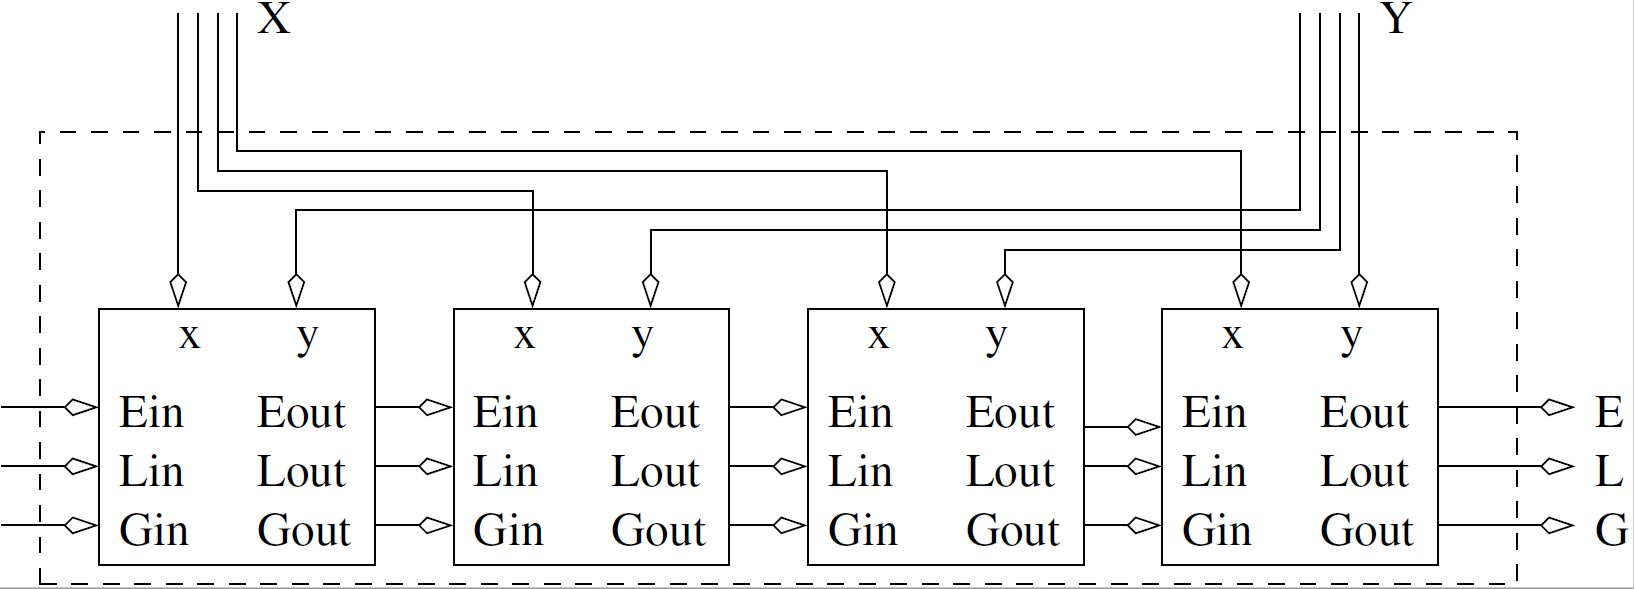
\includegraphics{./Fig2/compare.eps}
\vspace{0.3in}


\item {\bf (2 pt.)} How many address and data lines does a 1024x32 RAM have?
\vspace{0.3in}

\item{\bf (4 pts.)}
In the following question you are to complete the design of a counter with
the following truth atble and circuit diagram.  show how the signals are
routed to the mux.  

\begin{tabular}{lr}

\begin{tabular}[!t]{l|l|l||l}
clk         & $C_1 C_0$ & D & $Q^+$ \\ \hline \hline
0,1,$\downarrow$ & xx   & x & Q     \\ \hline
$\uparrow$     & 00     & x & Q     \\  \hline
$\uparrow$     & 01     & x & 0     \\  \hline
$\uparrow$     & 10     & x & Q+1 mod 16  \\  \hline
$\uparrow$     & 11     & D & D     \\
\end{tabular}
&
\scalebox{0.65}{\includegraphics[-20mm,90mm][0mm,0mm]{./Fig2/counter.eps}}
\end{tabular}

\pagebreak

\item {\bf (4 pts.)} Complete the timing diagram.

\scalebox{0.7}{\includegraphics{./Fig2/ExTim.eps}}

\item {\bf (4 pts.)} Write an equation describing the output.

\scalebox{0.7}{\includegraphics{./Fig2/TsbCircuit.eps}}
\vspace{0.3in}

\item {\bf (4 pts.)} Show the interconnections between a mux, a 
register and a counter to implement the following circuit.
\verb+if (X > Y) then Z = X else Z = Y;+
\vspace{0.3in}

\pagebreak
\item {\bf (4 pt.)}Describe the sequence of bits seen on the
$Q$ output.  Write down the output sequence until it starts to 
repeat.  Assume that $Q=0100$ initially.

\begin{tabular}{l|l|l|l||l|r}
clk         & $C_1 C_0$ & D & cin & $Q^+$ & comment \\ \hline \hline
0,1,$\downarrow$ & xx   & x & x   & Q     & hold     \\ \hline
$\uparrow$     & 00     & x & x   & Q     & hold     \\  \hline
$\uparrow$     & 01     & x & cin & $cin,Q_3,Q_2,Q_1$  & shift right \\  \hline
$\uparrow$     & 10     & x & cin & $Q_2,Q_1,Q_0,cin$  & shift left \\  \hline
$\uparrow$     & 11     & D & x   & D     & parallel load  \\ 
\end{tabular}

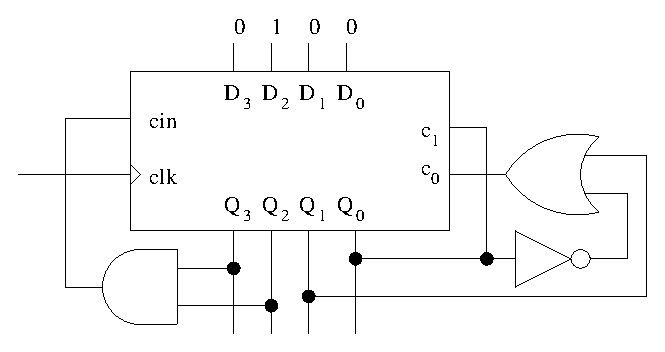
\includegraphics{./Fig2/shift.eps}
\vspace{0.3in}

\item{\bf (6 pts.)} Complete the timing diagram.

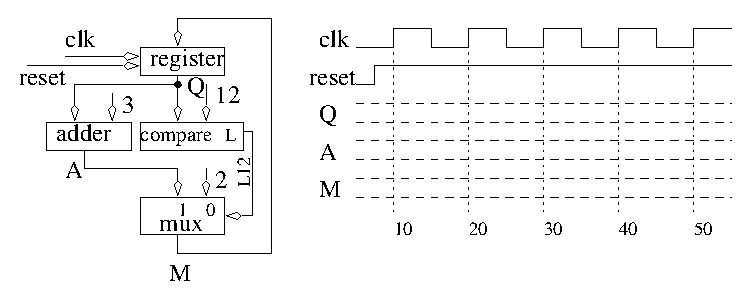
\includegraphics{./Fig2/BBBtiming1}

\end{enumerate}
\end{document}
